\section{GANs}

In this question, we are going to discuss GANs and their training process.

\subsection{GANs, a Game Theoretic Approach}

Game theory is a branch of mathematics that deals with the analysis of games. In this question, we are going to discuss GANs from a game theoretic approach. A game is defined by the following elements:

\begin{itemize}
    \item \textbf{Players:} The agents who are playing the game; row player and column player in a two-player game.
    \item \textbf{Actions:} The actions that each player can take; the strategies of each player.
    \item \textbf{Payoffs:} The rewards that each player receives based on the actions taken by all players; the utility function $u_i(a_1, a_2)$ for player $i$ in a two-player game where $a_1$ and $a_2$ are the actions taken by player 1 and player 2, respectively.
\end{itemize}

Nash Equilibrium is a concept in game theory that describes a situation in which no player can increase their payoff by changing their strategy, assuming that all other players keep their strategies unchanged. For example, in a two-player game, a Nash Equilibrium is a pair of strategies, one for each player, such that each player’s strategy is the best response to the other player’s strategy.

For example, consider a two-player game called Prisoner’s Dilemma. In this game, two players can either Cooperate or Defect. The payoffs for each player are as follows:
\begin{itemize}
    \item If both players Cooperate, they both receive a payoff of 3,
    \item If one player Cooperates and the other Defects, the player who Cooperates receives a payoff of 0, and the player who Defects receives a payoff of 5,
    \item If both players Defect, they both receive a payoff of 1.
\end{itemize}

We can define the Prisoner’s Dilemma as a game with the following matrix:

\begin{center}
\begin{tabular}{c|c|c}
 & Cooperate & Defect \\
\hline
Cooperate & 3,3 & 0,5 \\
\hline
Defect & 5,0 & 1,1 \\
\end{tabular}
\end{center}

Now, let's discuss how to find the Nash Equilibrium of a game. The Nash Equilibrium of a game can be found by solving the following optimization problem:

\[
\max_{a_1} \min_{a_2} u_1(a_1, a_2)
\]

\[
\max_{a_2} \min_{a_1} u_2(a_2, a_1)
\]

Where $a_1$ and $a_2$ are the actions taken by player 1 and player 2, respectively, and $u_1$ and $u_2$ are the payoffs of player 1 and player 2, respectively.

Now, let’s define GANs as a game. In a GAN, we have two players, the Generator and the Discriminator. The Generator tries to generate samples that are similar to the real data, while the Discriminator tries to distinguish between the real and generated samples.

\subsubsection{Question 1}

Define the GANs as a game. What are the players, actions, and payoffs in this game?
\begin{qsolve}
    \begin{qsolve}[]
        \textbf{Players:} The Generator and the Discriminator
        \begin{itemize}
            \item \textbf{Generator:} Tries to generate samples that are similar to the real data
            \item \textbf{Discriminator:} Tries to distinguish between the real and generated samples and maximize the probability of assigning the correct label to the samples
        \end{itemize}
        \textbf{Actions:} The actions that each player can take
        \begin{itemize}
            \item \textbf{Generator:} Generates fake samples from a noisy distribution
            \item \textbf{Discriminator:} Classifies the samples as real or generated to know a sample is fake or not
        \end{itemize}
        \textbf{Payoffs:} The rewards that each player receives based on the actions taken by all players
        \begin{itemize}
            \item \textbf{Generator:} The Generator receives a payoff based on how well the Discriminator is fooled by the generated samples
            \item \textbf{Discriminator:} The Discriminator receives a payoff based on how well it can distinguish between the real and generated samples
        \end{itemize}
    \end{qsolve}
\end{qsolve}
\subsubsection{Question 2}

To find the Nash Equilibrium of the GANs game, we need to solve the following optimization problem:

\[
\max_{\theta_G} \min_{\theta_D} u_G(\theta_G, \theta_D) = \max_{\theta_G} \min_{\theta_D} \mathbb{E}_{x \sim p_{\text{data}}} [\log D(x)] + \mathbb{E}_{z \sim p_z} [\log (1 - D(G(z)))]
\]

Explain this optimization problem and how it relates to the training process of the GANs.
\begin{qsolve}
    \begin{qsolve}[]
        The optimization problem of the GANs game is to find the Nash Equilibrium of the game. The Generator tries to minimize the probability of the Discriminator assigning the correct label to the generated samples, while the Discriminator tries to maximize the probability of assigning the correct label to the generated samples. The optimization problem is formulated as a minimax game, where the Generator minimize the loss function, and the Discriminator minimizes the loss function. the term $\mathbb{E}_{x \sim p_{\text{data}}} [\log D(x)]$ in the optimizationn problem represents the loss of the Discriminator when classifying the real samples and help it to maximize the probability of assigning the correct label to the real samples. 
        \splitqsolve[\splitqsolve]
        on the other hand the term $\mathbb{E}_{z \sim p_z} [\log (1 - D(G(z)))]$ represents the loss of the Discriminator when classifying the generated samples and help it to maximize the probability of assigning the correct label to the generated samples. training of GAN is as below:\\
        to train Discriminator, we first sample a batch of real data and a batch of fake data from the Generator. then we generate fake samples from current Generator and we calculate the loss function and update discriminator using GD to minimize the loss function.\\
        on the other hand to train the generator we generate fake samples from the current Generator and we calculate the loss function and update the Generator using GD to maximize the loss function.\\
        this training proccess will continue untill we reach the nash Equilibrium. this means that the Generator generates samples that are similar to the real data and the Discriminator can't distinguish between the real and generated samples.
    \end{qsolve}
\end{qsolve}
\subsubsection{Question 3}

To solve the optimization problem, we use the calculus of variations. Let $y = y(x)$ be a function of $x$ and the function we need to optimize is:

\[
\int F(x, y, y') \, dx
\]

For the function $y = y(x)$ that minimizes the integral, we know that:

\[
\frac{\partial F}{\partial y} - \frac{d}{dx} \left( \frac{\partial F}{\partial y'} \right) = 0
\]

You do not need to prove this formula. Now, solve the optimization problem of the GANs game using the calculus of variations. You need to find a closed-form solution for $\theta_D$.
\begin{qsolve}
    \begin{qsolve}[]
        the optimiazation problem of the GANs game is as below:
        \[
        \max_{\theta_G} \min_{\theta_D} u_G(\theta_G, \theta_D) = \max_{\theta_G} \min_{\theta_D} \mathbb{E}_{x \sim p_{\text{data}}} [\log D(x)] + \mathbb{E}_{z \sim p_z} [\log (1 - D(G(z)))]
        \]
        if we define $F(D(x))$ as below:
        \[
            F(D(x)) = p_{data}(x) \log D(x) + p_z(x) \log (1 - D(G(x))) 
        \]
        we can reformulate the optimization problem as below:
        \[
           \max_{\theta_G} \min_{\theta_D} \int F(D(x)) \, dx
        \]
        \splitqsolve[\splitqsolve]
        to find the optimal $\theta_D$ we need to solve the following equation:
        \[
            \frac{\partial F}{\partial D(x)} = 0
        \]
        so we have:
        \[
            \frac{\partial F}{\partial D(x)} = \frac{\partial}{\partial D(x)} (p_{data}(x) \log D(x) + p_z(x) \log (1 - D(x))) = 0
        \]
        \[
            \frac{\partial}{\partial D(x)} (p_{data}(x) \log D(x) + p_z(x) \log (1 - D(x))) = \frac{p_{data}(x)}{D(x)} - \frac{p_z(x)}{1 - D(x)} = 0
        \]
        \[
            \frac{p_{data}(x)}{D(x)} = \frac{p_z(x)}{1 - D(x)}
        \]
        \[
            \Rightarrow \theta_D = \frac{p_{data(x)}}{p_{data(x)} +p_z(x)}
        \]
    \end{qsolve}
\end{qsolve}
\subsection{GANs, You Don’t Want to Train Them!}

Training GANs is a challenging task due to the instability of the training process. In this question, we are going to discuss the challenges of training GANs. You can solve question 1 and 2 or you can solve question 3. NO extra points will be given for solving all three questions.

\subsubsection{Question 1}

Recall the optimization problem of the GANs game:

\[
\max_{\theta_G} \min_{\theta_D} u_G(\theta_G, \theta_D) = \max_{\theta_G} \min_{\theta_D} \mathbb{E}_{x \sim p_{\text{data}}} [\log D(x)] + \mathbb{E}_{z \sim p_z} [\log (1 - D(G(z)))]
\]

When using Gradient Descent to solve this optimization problem, the first term is the discriminator loss. When you update the parameters of the discriminator, if you take the gradient of the GANs loss with respect to the generator parameters, the first term will not be affected. Explain why the first term is not affected when updating the generator parameters. How does this affect the training process of GANs?
\begin{qsolve}
    \begin{qsolve}[]
        the objective function is as below:
        \[
        \max_{\theta_G} \min_{\theta_D} u_G(\theta_G, \theta_D) = \max_{\theta_G} \min_{\theta_D} \mathbb{E}_{x \sim p_{\text{data}}} [\log D(x)] + \mathbb{E}_{z \sim p_z} [\log (1 - D(G(z)))]
        \]
        when we take gradient of the GANs loss with respect to the discriminator parameters the equation will be:
        \[
            \nabla_{\theta_D} u_G(\theta_G, \theta_D) = \nabla_{\theta_D} \mathbb{E}_{x \sim p_{\text{data}}} [\log D(x)] + \nabla_{\theta_D} \mathbb{E}_{z \sim p_z} [\log (1 - D(G(z)))]
        \]
        \splitqsolve[\splitqsolve]
        but when we take gradient of the GANs loss with respect to the generator parameters the first term will not be affected. and the gradient will become:
        \[
            \nabla_{\theta_G} u_G(\theta_G, \theta_D) = \nabla_{\theta_G} \mathbb{E}_{z \sim p_z} [\log (1 - D(G(z)))]
        \]
        This is because the first term, $\mathbb{E}_{x \sim p_{\text{data}}} [\log D(x)]$, only involves real data samples and the discriminator's response to them. It does not depend on the generator parameters $\theta_G$. The generator does not directly influence how real data is classified by the discriminator; it only affects the fake data generated from the noise $z \sim p_z$.
        The fact that the generator's update step does not affect the term involving real data means that during training, the generator only focuses on improving the generation of fake samples to fool the discriminator. Specifically:

        \begin{itemize}
            \item \textbf{Discriminator Update:} When updating the discriminator, both real and fake samples are considered, allowing the discriminator to learn to distinguish between real and generated data.
            \item \textbf{Generator Update:} When updating the generator, only the fake samples' term is involved. The generator improves by making the fake samples more realistic to decrease the discriminator's ability to distinguish them from real samples.
        \end{itemize}

        This separation ensures that the generator and discriminator are updated in a way that maintains the adversarial nature of the game. However, it can also lead to instability in training:

       \end{qsolve}
\end{qsolve}
\subsubsection{Question 2}

It's known that the training process of GANs is unstable and can suffer from the mode collapse problem. Explain the mode collapse problem and how it affects the training process of GANs.
\begin{qsolve}
    \begin{qsolve}[]
        The mode collapse problem in GANs occurs when the generator produces a limited variety of outputs, often focusing on a few modes of the data distribution while ignoring others. This leads to a lack of diversity in generated samples, causing the generator to repeatedly generate similar outputs. As a result, the discriminator quickly learns to distinguish between real and generated samples, making training unstable. Mode collapse prevents the generator from learning the true data distribution and hinders the overall effectiveness of the GAN.
    \end{qsolve}
\end{qsolve}
\subsubsection{Question 3}

If you solve the optimization problem of the GANs for the optimal Discriminator, you will get the following optimization problem:

\[
u_D(\theta_G, \theta_D) = 2 D_{JS}(p_{\text{data}} \| p_{\text{model}}) - 2 \log(2)
\]

\[
= \frac{1}{2} D_{KL}(p_{\text{data}} \| \frac{p_{\text{data}} + p_{\text{model}}}{2}) + \frac{1}{2} D_{KL}(p_{\text{model}} \| \frac{p_{\text{data}} + p_{\text{model}}}{2}) - 2 \log(2)
\]

Where $D_{JS}$ is the Jensen-Shannon divergence, $D_{KL}$ is the Kullback-Leibler divergence (if you aren't familiar with KL divergence, it's a measure of how one probability distribution is different from a second, reference probability distribution).

Another problem with training GANs is the KL divergence term in the loss function. For better intuition, check the following image:

\begin{figure}[H]
    \centering
    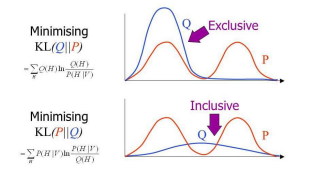
\includegraphics[width=0.5\textwidth]{gan_problem.png}
    \caption{ $p(x)$, the data distribution and $q(x)$, model distribution}
\end{figure}


To solve this problem, we can use Wasserstein GANs (WGANs) that replace the KL divergence term with the Wasserstein distance. Explain the Wasserstein distance and how it solves the problem of the KL divergence term in the loss function of GANs.
